\documentclass{standalone}
\usepackage{tikz}
\usetikzlibrary{decorations.pathreplacing}
\usepackage{amsfonts}

\begin{document}
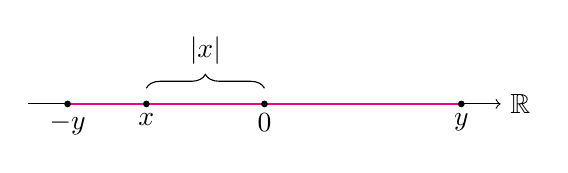
\begin{tikzpicture}
% Draw the real line
  \draw[->] (-3,0) -- (3,0) node[right] {$\mathbb{R}$};
  
  
  
    % Draw the red segment between '-y' and 'y' and make it thicker
  \draw[magenta, line width=1pt] (-2.5,0) -- (2.5,0);
  
  
  % Draw the point 'x' and '0'
  \filldraw (0,0) circle (1pt) node[below] {0};
  \filldraw (2.5,0) circle (1pt) node[below] {$y$};
  \filldraw (-2.5,0) circle (1pt) node[below] {$-y$};
  \filldraw (-1.5,0) circle (1pt) node[below] {$x$};
  
  % Draw the brace and label it
  \draw[decorate,decoration={brace,amplitude=5pt}] (-1.5,0.2) -- (0,0.2) node[midway,above=5pt] {$|x|$};
  

  
 
  
  
  
  \end{tikzpicture}
\end{document}